	\documentclass[12pt]{article}

%% Language and font encodings
\usepackage[english]{babel}
\usepackage[utf8x]{inputenc}
\usepackage[T1]{fontenc}

%% Sets page size and margins
\usepackage[a4paper,top=2cm,bottom=2cm,left=2cm,right=2.5cm,marginparwidth=1.75cm]{geometry}

%% Useful packages
\usepackage{amsmath}
\usepackage{amsfonts}
\usepackage{graphicx}
\usepackage[colorinlistoftodos]{todonotes}
\usepackage[colorlinks=true, allcolors=blue]{hyperref}

\title{Homework 6}
\author{Motoaki Takahashi}
\date{}

\begin{document}
\maketitle
\section*{Question 1}
Given the initial stock of lumber $k_{0}$, let $\mathcal{K}=[0, k_{0}]$ be the set of possible values for a stock of lumber, and  let $\mathcal{P}=\mathbb{R}$ be the set of possible prices. $\mathcal{K}\times\mathcal{P}$ is the state space. Let $(k, p)\in\mathcal{K}\times\mathcal{P}$. Then the Bellman equation is
\begin{equation}
    V(k, p)=\max_{k'} p\cdot (k-k')-0.2(k-k')^{1.5}+\delta\mathbb{E}_{p'\mid p}V(k', p')
\end{equation}
subject to
$$
p'=p_{0}+\rho p+u,\, u\sim N(0, \sigma_{u}^{2}),
$$
and
$$
k'\in[0, k].
$$
\section*{Question 2}
The vector of grids is $(0.6536,    0.6882,    0.7229,    0.7575,    0.7922,    0.8268,    0.8614, \cdots, 1.3118,    1.3464)$.
\clearpage
\section*{Question 3}
\begin{figure}[h]
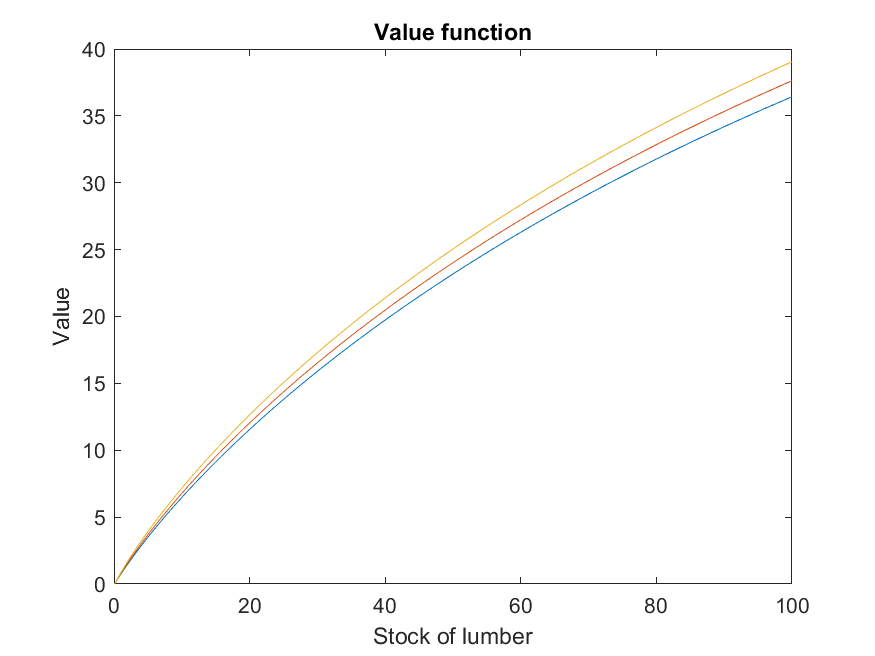
\includegraphics[width=\textwidth]{vf.png}
\caption{The values as a function of lumber stocks, for $p=0.9, 1, 1.1$}
\end{figure}
\clearpage
\section*{Question 4}

\begin{figure}[h]
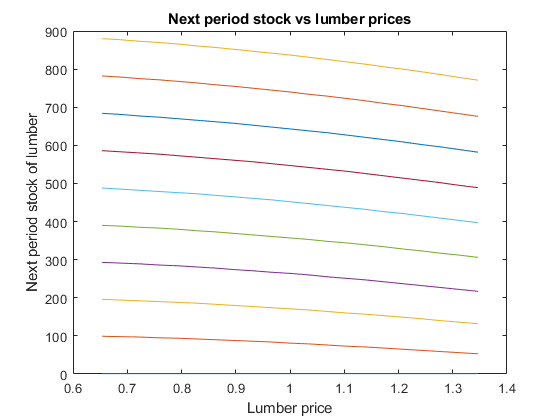
\includegraphics[width=\textwidth]{nextstock.png}
\caption{Next period optimal stocks as a function of lumber prices, for current period stock 0.1, 10.1, 20.1, ..., 90.1}
\end{figure}

\clearpage
\section*{Question 5}
\begin{figure}[h]
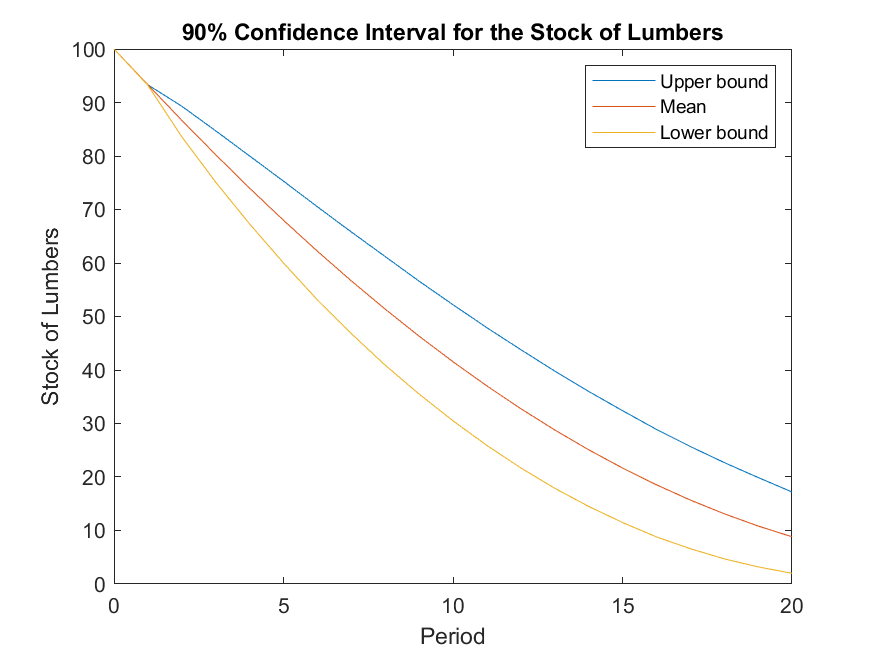
\includegraphics[width=\textwidth]{ci.png}
\caption{Expected stock and 90\% confidence interval}
\end{figure}
\clearpage
\section*{Question 6}
Since $p=0.9, 1.1$ are not on the grid, I draw two curves associated with the closest prices to them in Fig. 4.
\begin{figure}[h]
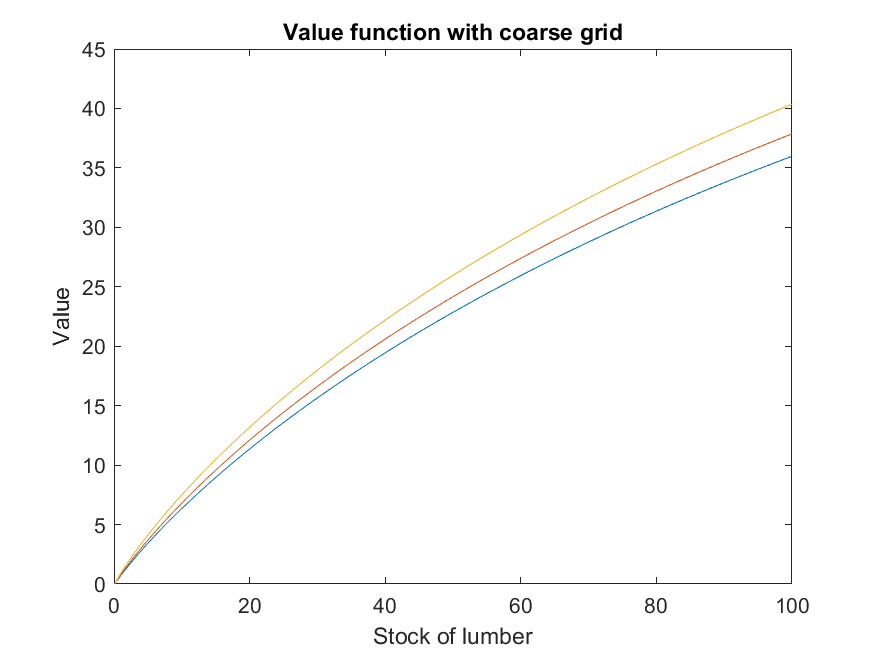
\includegraphics[width=\textwidth]{vf2.png}
\caption{The values as a function of lumber stocks, for $p=0.827, 1, 1.173$}
\end{figure}
\clearpage
\begin{figure}
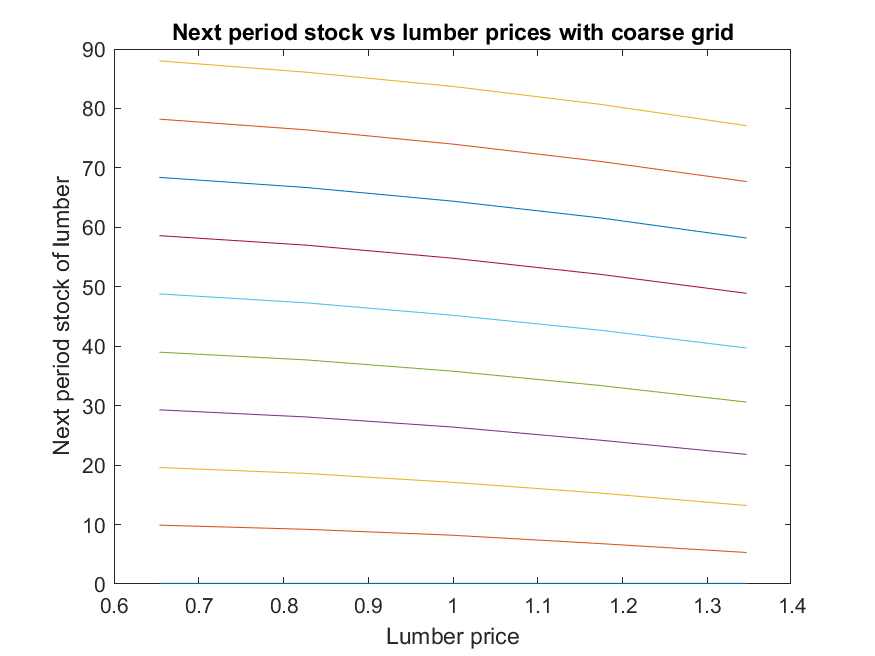
\includegraphics[width=\textwidth]{nextstock2.png}
\caption{Next period optimal stocks as a function of lumber prices, for current period stock 0.1, 10.1, 20.1, ..., 90.1}
\end{figure}
\clearpage
\begin{figure}[h]
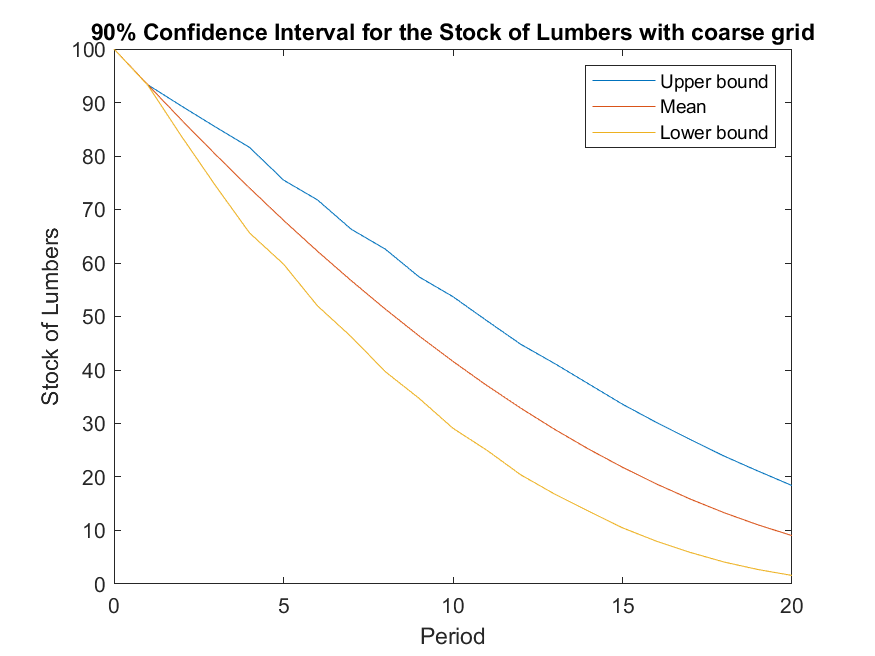
\includegraphics[width=\textwidth]{ci2.png}
\caption{Expected stock and 90\% confidence interval}
\end{figure}
\end{document}